\subsection{Predicting Performance Impact}

\label{sec:predictimprove}

%Fixing false sharing problems can be non-trivial, even with precise information about a particular false sharing problem. Several problems may occur. The first problem is that some false sharing problems can be insignificant. For example, \sheriff{} reports false sharing problems in word\_count or reverse\_index applications in Phoenix benchmark suites. However, fixing  them brings negligible performance benefit. The second problem is that fixing false sharing problem may even slow down the program because of excessive memory consumption or lose of locality, as observed by Zhao et. al. ~\cite{qinzhao}. 

We have discussed the basic idea of predicting performance impact of false sharing instances in Section~\ref{sec:predictidea}. This section focuses on the detailed algorithm of prediction. \Cheetah{} currently only predicts the performance impact of false sharing in programs with the normal fork-join model that does not have nesting threads. This normal fork-join model, shown as Figure~\ref{fig:forkjoinmodel}, is the most popular model in multithreading applications, as evidenced by all evaluated applications. 

\begin{figure*}[ht!]
\begin{center}
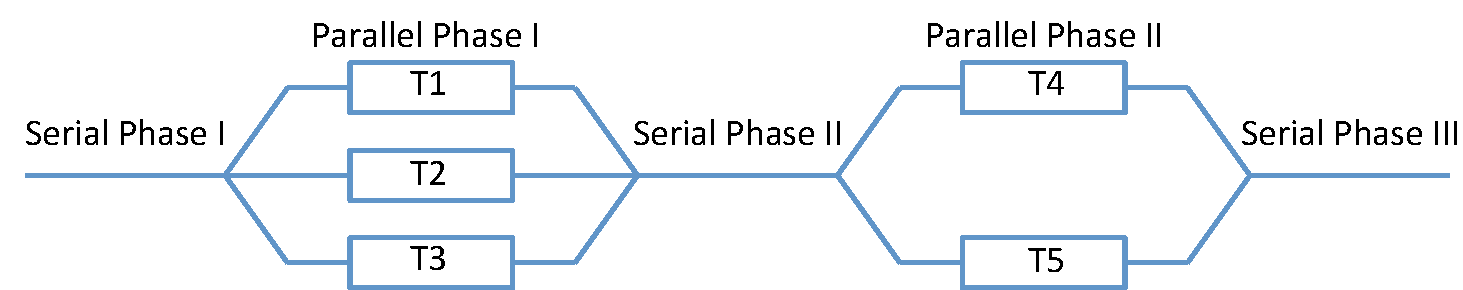
\includegraphics[width=6.5in]{figure/forkjoin}
\end{center}
\caption{\Cheetah{} can predict the performance impact of false sharing inside applications with normal fork-join model.
\label{fig:forkjoinmodel}}
\end{figure*}

%We will talk about how to get 

\subsection{Getting Actual Execution Time}
\label{sec:getactualtime}

According to EQ.(\ref{eq:improvement}), to compute the performance improvement, we have to get the actual execution time ($RT_{actual}$). 
\fixme{For simplicity, \cheetah{} collects the actual execution time using RDTSC (ReaD-Time Stamp Counter) on X86 machines}.  \cheetah{} does not use access cycles of threads since the execution time can highly depends on how many threads are created and how they are running on different cores, which is too complicated to compute.  

To predict the performance impact of a false sharing instance, \Cheetah{} also tracks the relationship of different threads by maintaining a tree graph like the example shown in Figure~\ref{fig:forkjoinmodel}. \Cheetah{} also collects the execution time of different phases and different threads. Based on these information, \Cheetah{} can predict the performance impact of a certain false sharing instance. 
 
\subsection{Predicting Execution Time after Fixes}
\label{sec:predicttime}

As described in Section~\ref{sec:predictidea}, \cheetah{} predicts the execution time after fixes by replacing the actual cycles of every memory access on a falsely-shared object with the average cycles of a memory access without false sharing. Actually, those memory accesses related to true sharing should be ruled out as well since they are also much slower. 

According to this idea, \cheetah{} should know the average cycles of a memory access without false sharing and true sharing. To know exactly about this value, we have to compute the number of cycles of all memory accesses without false sharing and true sharing. But that is not easy. \Cheetah{} actually utilizes the average access cycles of every memory access in serial phases (denoted as $AverageCycles_{nofs}$) to approximate this value, which is reasonable since all memory accesses in serial phases should not involve in both false sharing and true sharing. 

Actual cycles of every memory access that are involving in a falsely-shared object can be changed from one execution to another. Thus, \cheetah{} utilizes the total number of all memory accesses instead to predict the performance impact. \Cheetah{} computes the possible performance improvement prediction in the following steps.
 
\begin{enumerate}
\item \cheetah{} first compute the total number of accesses ($Accesses_{fs}$) on suspected cache lines and the total cycles of accesses ($Cycles_{fs}$) on suspected cache lines.

\item For threads that are involved a particular false sharing, \cheetah{} then compute the total number of accesses ($Accesses_{threads}$) and the total cycle of accesses ($Cycles_{threads}$). 

\item \Cheetah{} computes the estimated cycles of those threads that are involved in false sharing according to the formula $Cycles_{pred} = Cycles_{threads} - Cycles_{fs} + Accesses_{fs} * AverageCycles_{nofs}$. 

\item  Based on this, \cheetah{} will compute the performance improvement on threads that are involved in false sharing.
$RT_{threads} = Cycles_{threads}  $. 

\end{enumerate}



\cheetah{} collects the actual execution time 
\cheetah{} will utilize the latency information of every access to predict the performance impact of a certain false sharing instance. These latency information, normally CPU cycles of every sampled memory access, can be provided by hardware PMUs. \Cheetah{} plans to track detailed memory accesses on falsely-shared objects and on normal objects without false sharing. Thus, we can know the average cycles of every memory access without false sharing. 

\cheetah{} provides a upper bound on performance improvement after fixes. 

It is note that sampling based approaches can actually 
.

We only compute the cycles and threads for the parallel phases. 

\subsection{Predicting Performance Improvement}

There are several steps to evaluate the performance impact. We will consider the average cycles on every access in serial phases as $Cycles_{serial}$. 

 % How to avoid huge performance overhead? We introducing per-thread recording mechanism. 

% How to actually predict the performance improvement? A thread may have the serial part and parallel part. We have to identify the serial part and parallel part. 

% How to handle different CPUs? For example, we may start 16 threads on 8 CPUs. 

% Can we get the resolute time on each phase? We are using this to calculate the performance improvement.  We also copy the whole memory accesses information out before transferring phases. 

% What if only two threads only accesses a specific cache line and other threads didn't accesses that? We can actually check the word level's accesses to find out those number of threads that are accesses this tid. We could also verify whether those memory accesses are on the critical path or not. 

% We should use actual tid instead of thread index to identify threads. 

% We should remove the write-invoked tracking since we have to check the number of accesses. Thus, we actually don't care those ones that are happened in the serial phase. Because we won't actual change its performance initially. 



% The total number of memory accesses on an addresses

% The total latency of accessing an address

% The total number of memory accesses for each thread. 

% The total latency of all memory accesses for each thread  

% All memory accesses of each thread

% All memory accesses in total = Sum of (memory accesses of each thread)

% Total latency of all memory accesses for each thread. 